\setTitle{CavalierCity}
\setGrade{5e}
\emptyBackground
\def\authors{Mme ANGOUILLANT et M. PESIN}
%%%%

\small

\section*{Mission : Aménagement urbain}
\vspace{-0.15cm}

Bienvenue dans votre nouvelle mission !
Vous avez été désigné comme responsable de l'aménagement urbain d'une toute nouvelle ville.
Votre objectif : imaginer et concevoir un espace harmonieux et fonctionnel qui saura séduire ses futurs habitants.

Pour cela, vous devrez :
\begin{itemize}
    \item Réaliser une carte précise de votre ville, détaillant l'emplacement des différentes rues, bâtiments et infrastructures.
    \item Construire une «maquette» sur papier en perspective cavalière qui permettra de visualiser votre projet en 3D.
    \item Trouver un nom unique et évocateur pour votre ville, qui reflète son identité et son ambiance.
\end{itemize}

Le conseil municipal, composé de Mme Angouillant et M. Pesin, attend avec impatience votre présentation.
Ce sont eux qui décideront si votre projet est retenu !
Bonne chance dans cette aventure créative et architecturale !
\vspace{-0.5cm}
\section*{Évaluation}
\vspace{-0.15cm}
En mathématiques, vous serez évalué sur :
\begin{itemize}
    \item la diversité des solides employés dans la construction de votre ville ;
    \item la précision de vos tracés, notamment la correspondance entre la carte et la «maquette».
\end{itemize}

\vspace{-0.5cm}
\section*{Travail préliminaire}
\vspace{-0.15cm}

Avant de commencer, réfléchissez aux points suivants :
\begin{enumerate}
    \item Souhaitez-vous suivre un thème spécifique ? 
    (Par exemple : une ville futuriste, médiévale, fantastique, etc.)
    \item Quels bâtiments voulez-vous intégrer dans votre ville ? 
    (Par exemple : un hôpital, une école, des maisons, etc.)
    \item Réalisez au brouillon, sur une feuille pointée en perspective cavalière, quelques bâtiments pour vous inspirer.
\end{enumerate}

\vspace{-0.5cm}
\section*{Procédure de construction}
\vspace{-0.75cm}

\begin{enumerate}
    \item Tracez la carte (empreinte) de votre ville sur le premier papier :
    \begin{tikzpicture}[scale = 0.05]
    \draw [dotted] (12,4.00) -- (32,4.00) -- (32,24.00) -- (12,24.00) -- (12,4.00);
\end{tikzpicture}
    \begin{itemize}
        \item Dessinez l'empreinte de votre ville et nommez les bâtiments que vous placez (en anglais).
        \item Ajoutez les noms de rues / places / etc (en anglais).
    \end{itemize}
    \item Construisez votre «maquette» sur le second papier :
    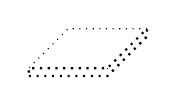
\begin{tikzpicture}[scale = 0.05]
    % \boundingBox[45][31.5][0.5pt][1][(0,-1)][cavalier][black!0]
    \draw [thick,dotted] (8,2) -- (28,2) -- (38,12) -- (38,14) -- (28,4) -- (8,4) -- (8,2);
    \draw [dotted] (28,4) -- (28,2);
    \draw [dotted] (38,14) -- (18,14) -- (8,4);
\end{tikzpicture}
    \begin{itemize}
        \item Reproduisez l'empreinte de votre ville au crayon à papier.
        \item Dessinez, toujours au crayon à papier, les solides correspondant à vos bâtiments en respectant les proportions.
        \item Effacez les traits cachés (ceux qui se trouvent derrière un bâtiment ou à l'intérieur d'une structure complexe).
    \end{itemize}
    \item Laissez libre cours à votre imagination : ajoutez des détails et de la couleur à vos bâtiments comme bon vous semble ! 
    Ne vous inquiétez pas si certains détails cachent partiellement vos bâtiments, cela ne sera bien sûr pas pénalisé.
\end{enumerate}
